\noindent

\includegraphics[height=1.25cm]{images/pictograms/replication}
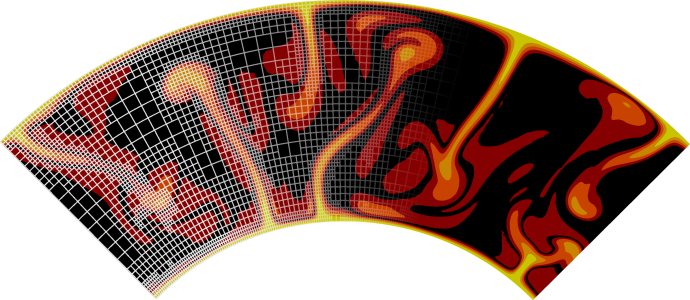
\includegraphics[height=1.25cm]{images/pictograms/aspect_logo}

\includegraphics[height=1.25cm]{images/pictograms/benchmark}

\includegraphics[height=1.25cm]{images/pictograms/under_construction}

\includegraphics[height=1.25cm]{images/pictograms/FEM}

\includegraphics[height=1.25cm]{images/pictograms/paraview}

%%%%%%%%%%%%%%%%%%%%%%%%%%%%%%%%%%%%%%%%%%%%%%%%%%%%%%%%%%%%%%%%%%%%%%%%%%%%%%%%%%%%%%%%%%%%%%%%%%%

\begin{flushright} {\tiny {\color{gray} python\_codes/fieldstone\_160/text.tex}} \end{flushright}

%\lstinputlisting[language=bash,basicstyle=\small]{python_codes/template_keywords.key}

\par\noindent\rule{\textwidth}{0.4pt}

\begin{center}
\inpython
{\small Code: \url{https://github.com/cedrict/fieldstone/tree/master/python_codes/fieldstone_160}}
\end{center}

\par\noindent\rule{\textwidth}{0.4pt}

{\sl This stone was developed in collaboration with J.C. Afonso}. \index{contributors}{J.C. Afonso}

\par\noindent\rule{\textwidth}{0.4pt}


%%%%%%%%%%%%%%%%%%%%%%%%%%%%%%%%%%%%%%%%%%%%%%%%%%%%%%%%%%%%%%%%%%%%%%%%%%%%%%%%%%%%%%%%%%%%%%%%%%%


There are three materials in the domain:
\begin{itemize}
\item crust: $\rho_{c}=2300~\si{\kg\per\cubic\meter}$ and $\eta_{c}=10^{23}~\si{\pascal\second}$;
\item mantle: $\rho_{m}=3300~\si{\kg\per\cubic\meter}$ and $\eta_{c}=10^{21}~\si{\pascal\second}$;
\item weak zones: $\rho_{wz}=\rho_{c}$ and $\eta_{wz}=10^{-3}\eta_{c}$.
\end{itemize}
The domain is a Cartesian box of size $L_x=120~\si{\km}$, $L_y=100~\si{\km}$.
Free slip boundary conditions are imposed on all four sides. ${\bm Q}_2 \times Q_1$ 
(continuous pressure)
or ${\bm Q}_2\times P_{-1}$ (discontinuous pressure) elements are used.
The crust is 20~\si{\km} thick but is thickened (40~\si{\km} depth) in the middle 30~\si{\km}.
On each side we find weak zones as thick as the crust and 1~\si{\km} wide. 
The default resolution is set to 120$\times$1200 elements.

The boundary conditions are such that the pressure is computed up to a constant (null space)
and it is therefore normalised by imposing that the average pressure at the surface is zero.

\begin{center}
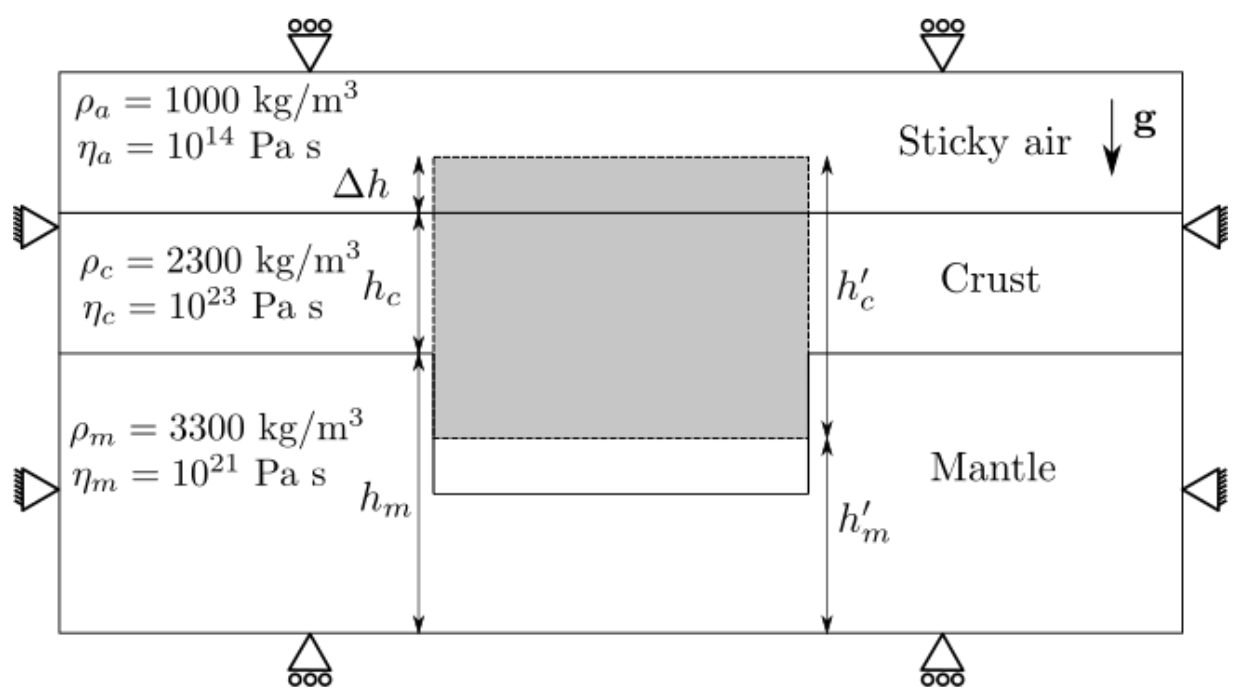
\includegraphics[width=9cm]{python_codes/fieldstone_160/images/setup}\\
{\captionfont Figure by J.C. Afonso. $h_c$ and $h_m$ are the initial thicknesses of the crust and 
mantle. $h_c'$ is the thickness of the thickened crust, and $h_m'$ is the thickness of the 
mantle below the thickened crust at isostatic equilibrium. Drawing not to scale.}
\end{center}


The thickened crust has a positive buoyancy with respect to the normal crust due
to density difference, whose analytical value is found via a standard isostatic balance (i.e.
equating the mass per unit area of two columns at the compensation level, here taken at
the base of the numerical domain).




On the left or right sides, the lithostatic pressure at the base of the crust is then 
$\rho_{c} g h_{c}=2300*10*20000=460~\si{\mega\pascal}$.
At the base of the model, then the pressure is $450e6+\rho_{m} g h_{m}
=450e6+3300*10*80000=450e6+2640e6=3090~\si{\mega\pascal}$.
In a more abstract way, $P_{bottom}=\rho_c g h_c + \rho_m g h_m$.
In the middle, after the block has moved up and is now in isostatic equilibrium, 
we should have $P_{bottom}=\rho_c g h_c' + \rho_m g h_m'$.
In the end:
\[
P_{bottom}=\rho_c g h_c + \rho_m g h_m = \rho_c g h_c' + \rho_m g h_m'
\]
We can divide both sides by $g$:
\[
\rho_c  h_c + \rho_m  h_m = \rho_c  h_c' + \rho_m  h_m'
\]
\[
\Rightarrow \rho_m h_m'= \rho_c(h_c-h_c') + \rho_m h_m 
\]
\[
\Rightarrow h_m'=h_m-(h_c'-h_c)\frac{\rho_c}{\rho_m} 
\]
Then
\begin{eqnarray}
\Delta h 
&=& h_c' + h_m' - h_c - h_m \nn\\
&=& h_c' + h_m -(h_c'-h_c)\frac{\rho_c}{\rho_m} -h_c - h_m \nn\\
&=& h_c'  -(h_c'-h_c)\frac{\rho_c}{\rho_m} -h_c  \nn\\
&=& (h_c'-h_c)  -(h_c'-h_c)\frac{\rho_c}{\rho_m}   \nn\\
&=& (h_c'-h_c) \left(1 -\frac{\rho_c}{\rho_m} \right) 
\end{eqnarray}
Substituting for the parameters of our example, the predicted topography uplift is 
\[
\Delta h = (40000-20000)*(1-2300/3300) \simeq 6060~\si{\meter}
\]


In the \aspect manual we find the following documentation for the 'dynamic topography' post-processor:
``
A postprocessor that computes a measure of dynamic topography based on the stress at the boundary. 
The exact approach works as follows: At each selected boundary, we compute the traction that acts normal to 
the boundary faces using the consistent boundary flux method as described in \textcite{grls87}
From this traction, the dynamic topography is computed using the formula $h=\sigma_n / \rho g$ where $g$
is the norm of the gravity and $\rho$
is the density. For the bottom surface we chose the convention that positive values are up and negative values are down, 
analogous to the deformation of the upper surface. Note that this implementation takes the direction of 
gravity into account, which means that reversing the flow in backward advection calculations will not reverse 
the instantaneous topography because the reverse flow will be divided by the reverse surface gravity. 
''

In practice the dynamic topography is then computed as follows: 
\[
h= \frac{\vec{n} \cdot {\bm \sigma}\cdot \vec{n}}{\rho_c g } 
= \frac{\sigma_{yy}}{\rho_c g}
= \frac{-p+\tau_{yy}}{\rho_c g}
\]
where $\vec{n}$ is the normal vector to the surface\footnote{$\vec{t} ={\bm\sigma}\cdot \vec{n}$ 
is the traction on the boundary and then $\vec n \cdot \vec t$ is the component of this traction
along the normal.}. 


\begin{center}
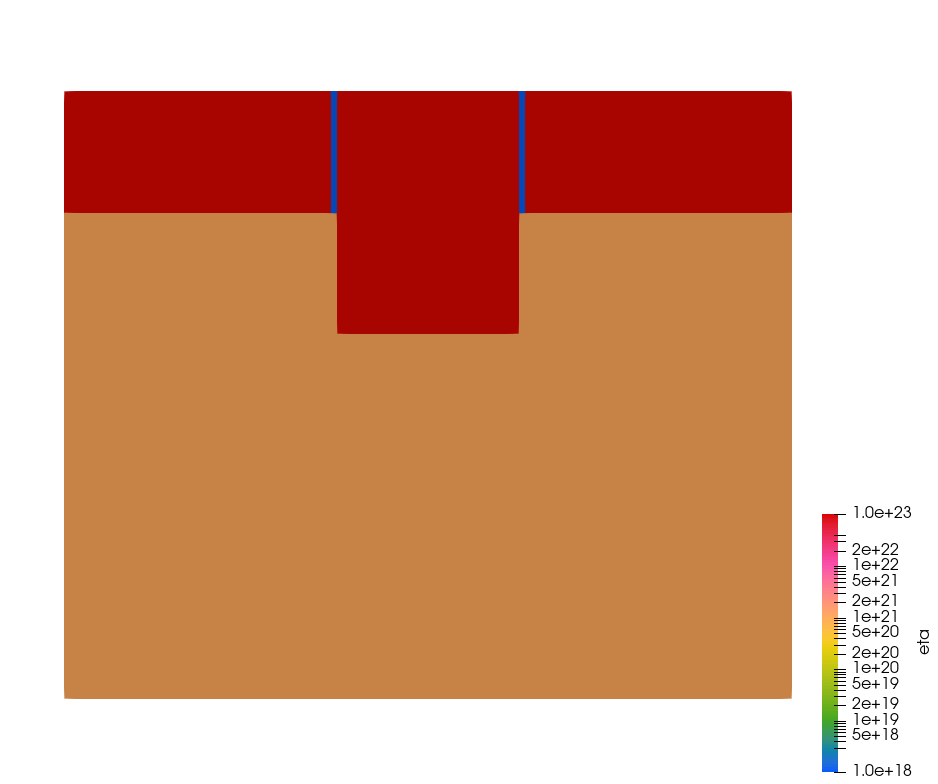
\includegraphics[width=8cm]{python_codes/fieldstone_160/results/eta.png}

\includegraphics[width=8cm]{python_codes/fieldstone_160/results/rho.png}\\
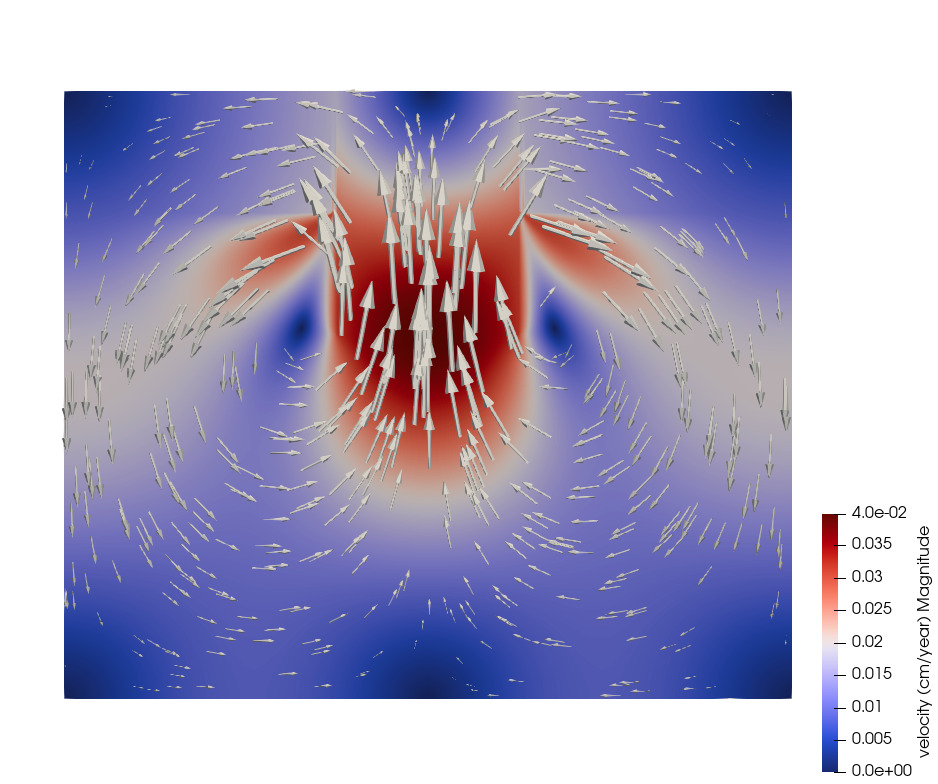
\includegraphics[width=8cm]{python_codes/fieldstone_160/results/vel.png}

\includegraphics[width=8cm]{python_codes/fieldstone_160/results/press.png}\\
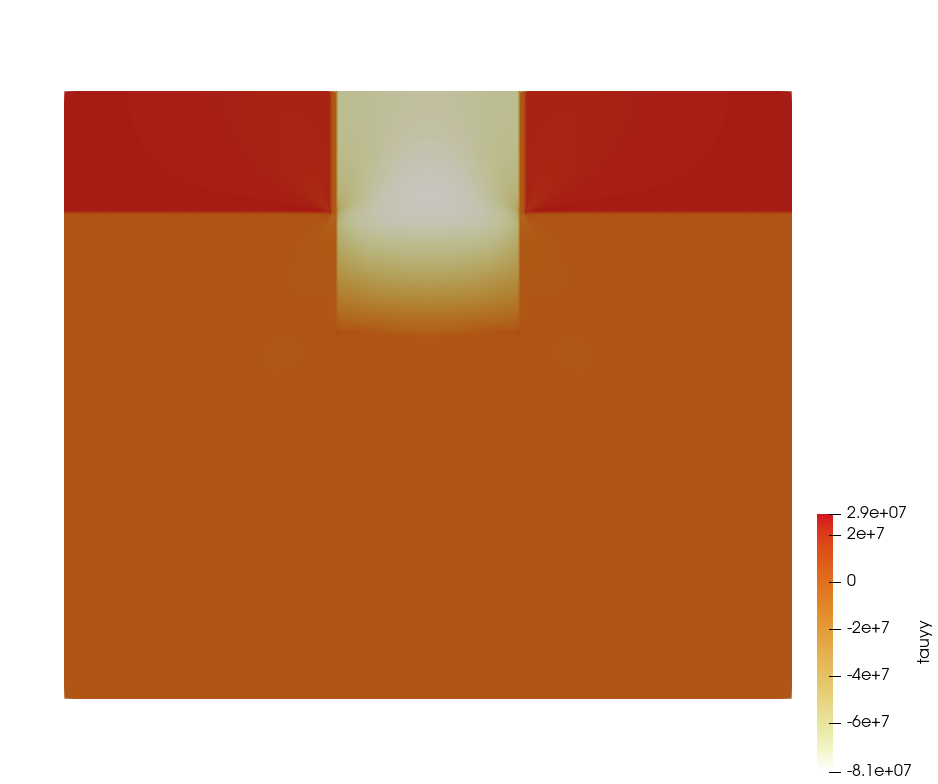
\includegraphics[width=8cm]{python_codes/fieldstone_160/results/tau_yy.png}
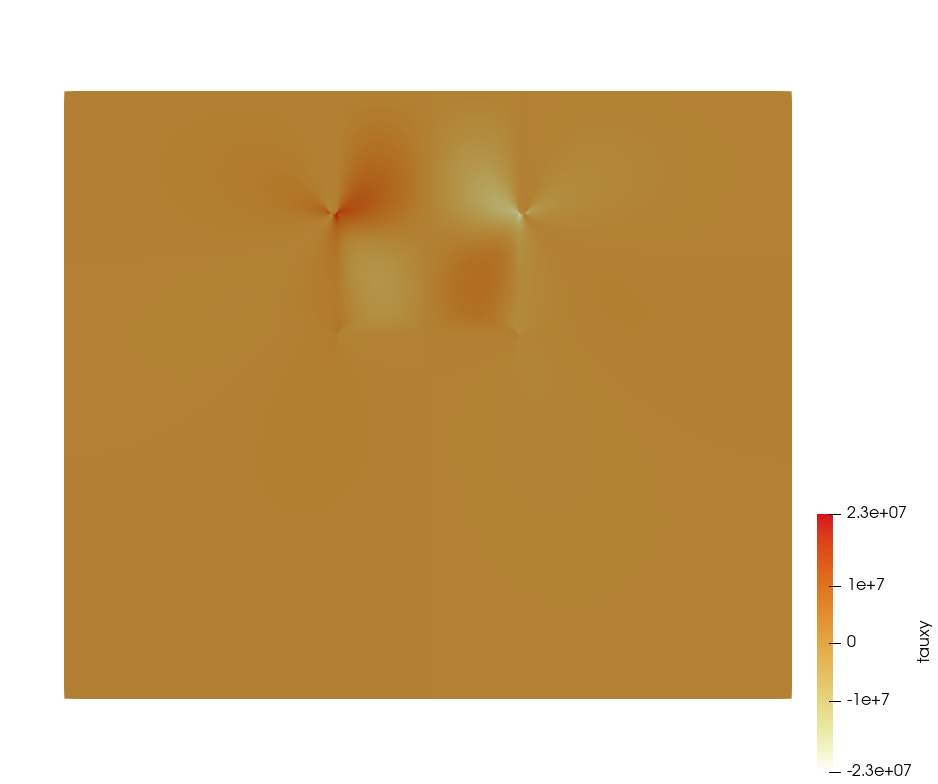
\includegraphics[width=8cm]{python_codes/fieldstone_160/results/tau_xy.png}\\
{\captionfont Results obtained on 240x200 mesh.}
\end{center}



The surface pressure, $yy$ component of deviatoric stress ${\bm \tau}$ 
and dynamic topography are shown in th following plots
\begin{center}
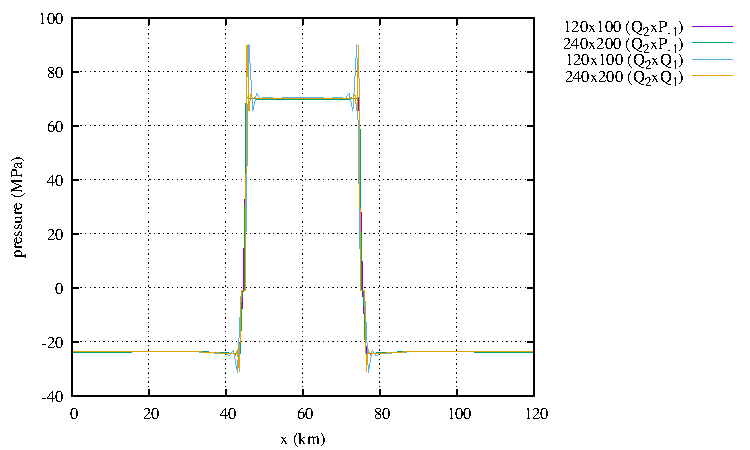
\includegraphics[width=8cm]{python_codes/fieldstone_160/results/pressure.pdf}
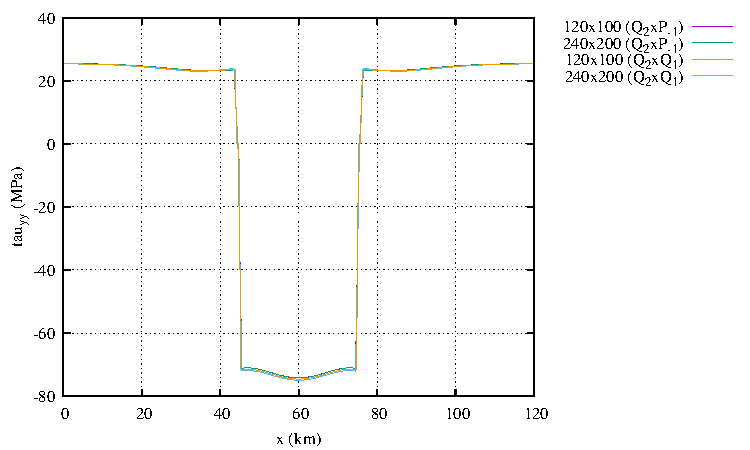
\includegraphics[width=8cm]{python_codes/fieldstone_160/results/tau_yy.pdf}\\
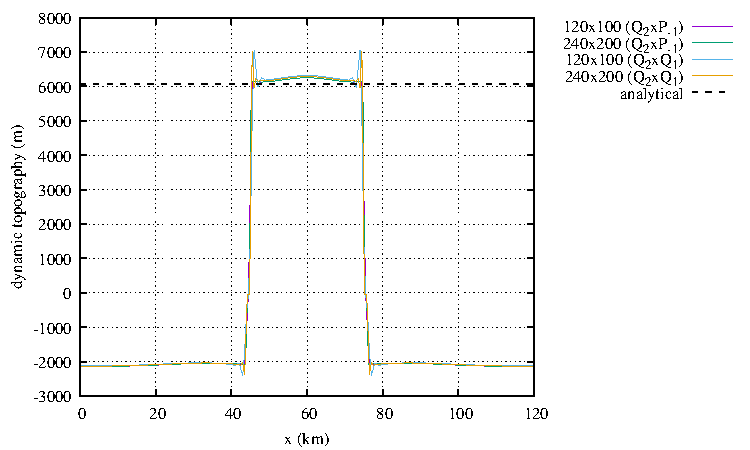
\includegraphics[width=8cm]{python_codes/fieldstone_160/results/dyn_topo.pdf}
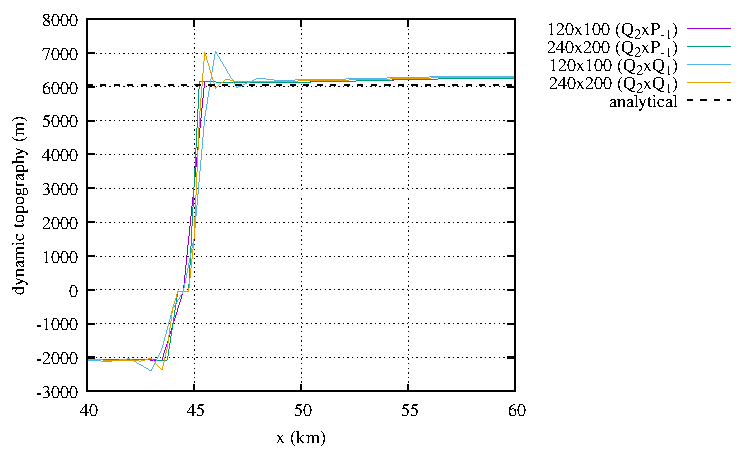
\includegraphics[width=8cm]{python_codes/fieldstone_160/results/dyn_topo2.pdf}
\end{center}
We find that the differences between low and high resolution are really small. 
The recovered dynamic topography is very close to the expected analytical value,
but since its accuracy is not improving with resolution this probably means that the 
weak zones and/or the coupling of the keel of the crust with the mantle is 
playing a role.
We also find that the discontinuous pressure element unsurprisingly copes better 
with the element boundary-aligned viscosity jumps, while the continuous pressure 
one yields overshoots on the pressure field.

Let us now investigate the influence of the weak zones viscosity on the 
dynamic topography (zoomed on the important part):
\begin{center}
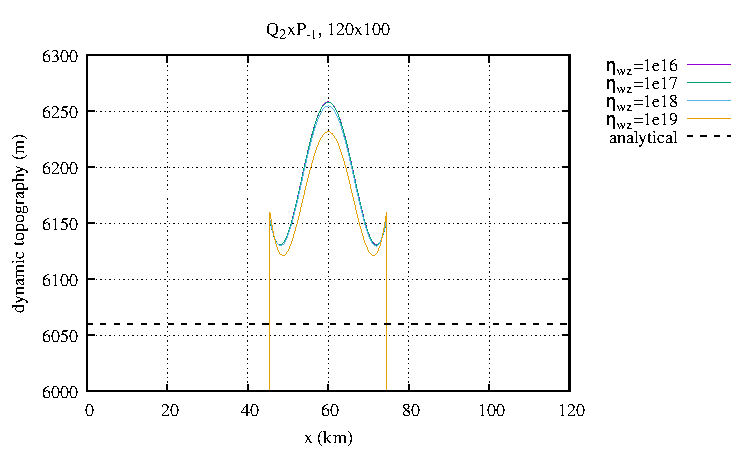
\includegraphics[width=8cm]{python_codes/fieldstone_160/results/dyn_topo3a.pdf}
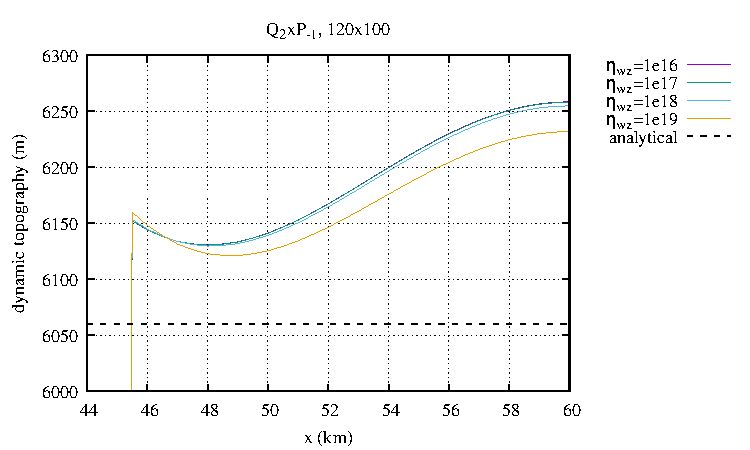
\includegraphics[width=8cm]{python_codes/fieldstone_160/results/dyn_topo3b.pdf}
\end{center}
The default value of $1e18$ is clearly low enough since lower values do not 
yield any visible change. This means that the signal we observe is entirely due
to the geometry of the experiment and the coupling crust keel-mantle.

We can now look at the influence of the mantle viscosity:
\begin{center}
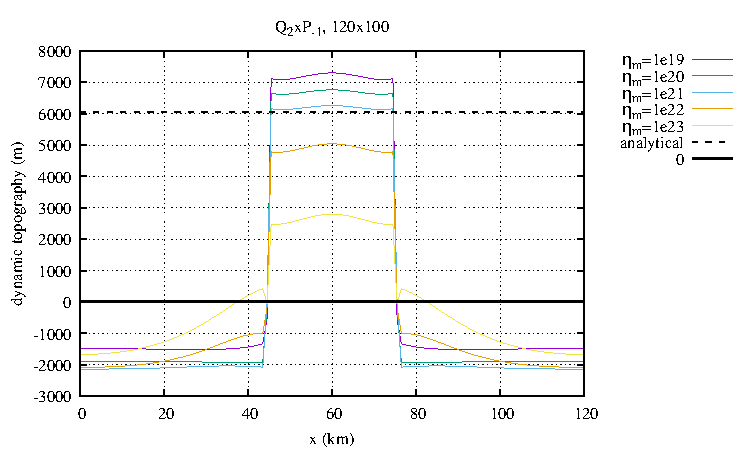
\includegraphics[width=8cm]{python_codes/fieldstone_160/results/dyn_topo4a.pdf}
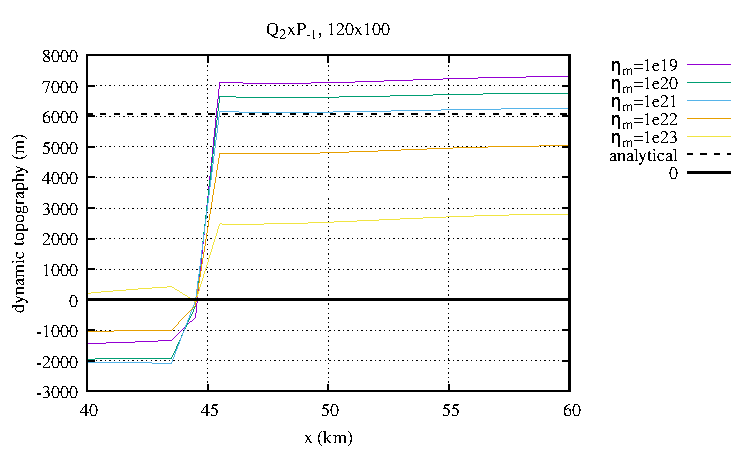
\includegraphics[width=8cm]{python_codes/fieldstone_160/results/dyn_topo4b.pdf}
\end{center}


